\documentclass{beamer}
\title{Decision Rule Approach with Transformation Technique}
\author{Zhan Lin\\linzhan@mail.ustc.edu.cn}
\begin{document}
\maketitle
\begin{frame}
\frametitle{Original Problems}

\begin{block}{}
\begin{equation}
\begin{array}{ll}
\max\limits_{\mathbf{x_t}} &\mathbb{E}_{\xi}\left(\sum\limits^T_{t=1} \mathbf{v}^T \mathbf{x_t} \left(\xi^{t-1},\xi_t\right)\right)\\
s.t. & \sum\limits^T_{t=1} A \mathbf{x_t} \left(\xi^{t-1},\xi_t\right) \leq \mathbf{c}\\
& \mathbf{x_t}(\xi^{t-1},\xi_t) \geq 0\\
&\forall \xi \in \Xi,t=1,\ldots,T
\end{array}
\label{origin}
\end{equation}
\end{block}
\begin{itemize}
\item
Capacity levels $\mathbf{c}=(c_1,\ldots,c_m)^T$.
\item
Corresponding prices $\mathbf{v} = (v_1,\ldots,v_n)^T$.
\item
Each products needs at most one unit of each resource. Let $A = \left(a_{ij}\right)$ be the resource coefficient matrix.
\item
$\xi_t$ is demands on period t and $\xi^{t-1}$ is information of demands before period t.
 \end{itemize}
\end{frame}
\begin{frame}
\frametitle{Transformation}

\begin{block}{}
\begin{equation}
\begin{array}{ll}
\max\limits_{\mathbf{\mathcal{X}_t}} &\mathbb{E}_{\xi}\left(\sum\limits^T_{t=1} \mathbf{v}^T \mathbf{\mathcal{X}_t}\left(\xi^{t-1},\xi_t\right)\right)\\
s.t. & \mathcal{X}_t(\xi^{t-1},\xi_t) \leq \xi_t\\
& \{\mathbf{\mathcal{X}_t}(\xi^{t-1},\xi_t) = (\mathcal{X}_{t,1}(\xi^{t-1},\xi_{t,1}),\mathcal{X}_{t,2}(\xi^{t-1},\xi_{t,2})\ldots\\
&,\mathcal{X}_{t,j}(\xi^{t-1},\xi_{t,j}))^T\}\in \mathcal{F}  \\
&\forall \xi \in \Xi,t=1,\ldots,T
\end{array}
\label{originsec}
\end{equation}
where $\mathcal{F}=\{\{f(\xi^{t-1},\xi_t)\}:f(\xi^{t-1},\xi_t) = \mathbf{u}_t(\xi^{t-1})\bigwedge \xi_t,\mathbf{u_t}(\xi^{t-1})\in\mathbb{R}^+,\sum\limits^T_{t=1} A \mathbf{u_t}(\xi^{t-1})\leq \mathbf{c}\}$.
\end{block}
\end{frame}
\begin{frame}{}
\frametitle{Functional Optimization}
\begin{itemize}
\item How to optimize object with $\{\mathcal{X}_t(\xi^{t-1},\xi_t)\} \in \mathcal{F}$?
\item How to implement polices when we have no knowledge of $\xi_{t}$?
\item As lower time complexity as possible with acceptable numerical accuracy.
\end{itemize}

\begin{figure}
\centering
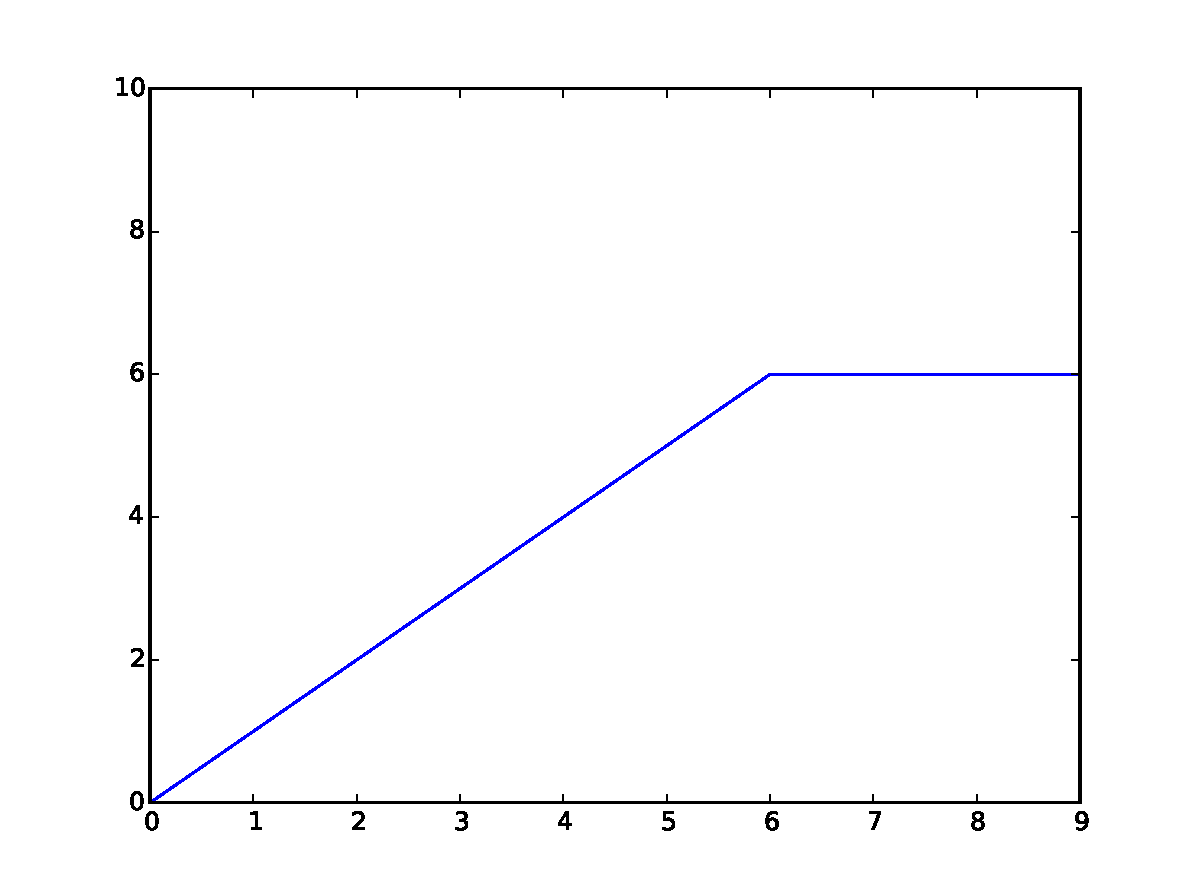
\includegraphics[width=.6\textwidth]{plf_1.pdf}
\caption{values of $\mathcal{X}_t(\xi^{t-1},\xi_t)$ when $\xi_t$ varies and keep $\xi^{t-1}$}\label{plf:1}
\end{figure}

\end{frame}

\begin{frame}
\frametitle{Generalized Decision Rule Approach}
Put decisions as a linear combination of historic information?

No! Put it as a linear combination of basis functions!
\begin{columns}
\column{.5\textwidth}
\begin{figure}
\flushright
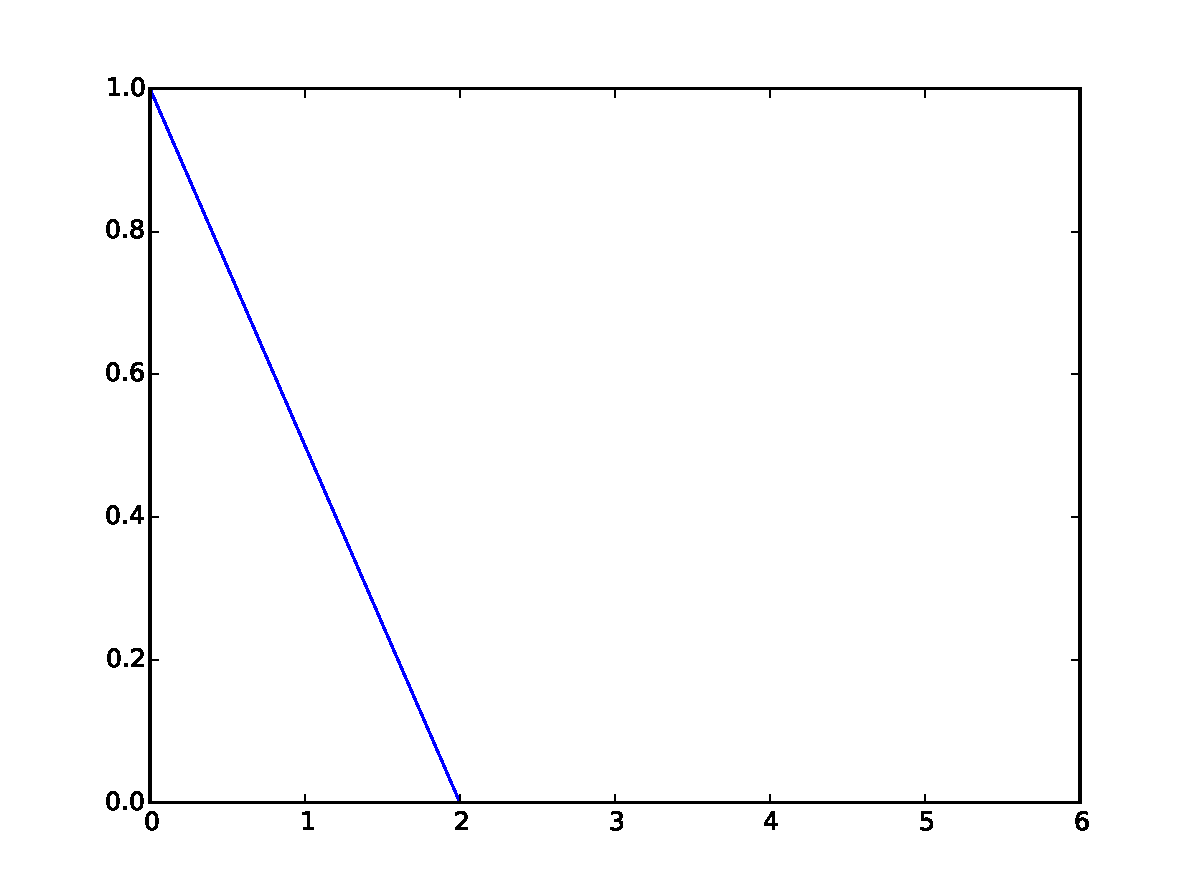
\includegraphics[width=.7\textwidth]{basis_1.pdf}
\end{figure}
\column{.5\textwidth}
\begin{figure}
\flushleft
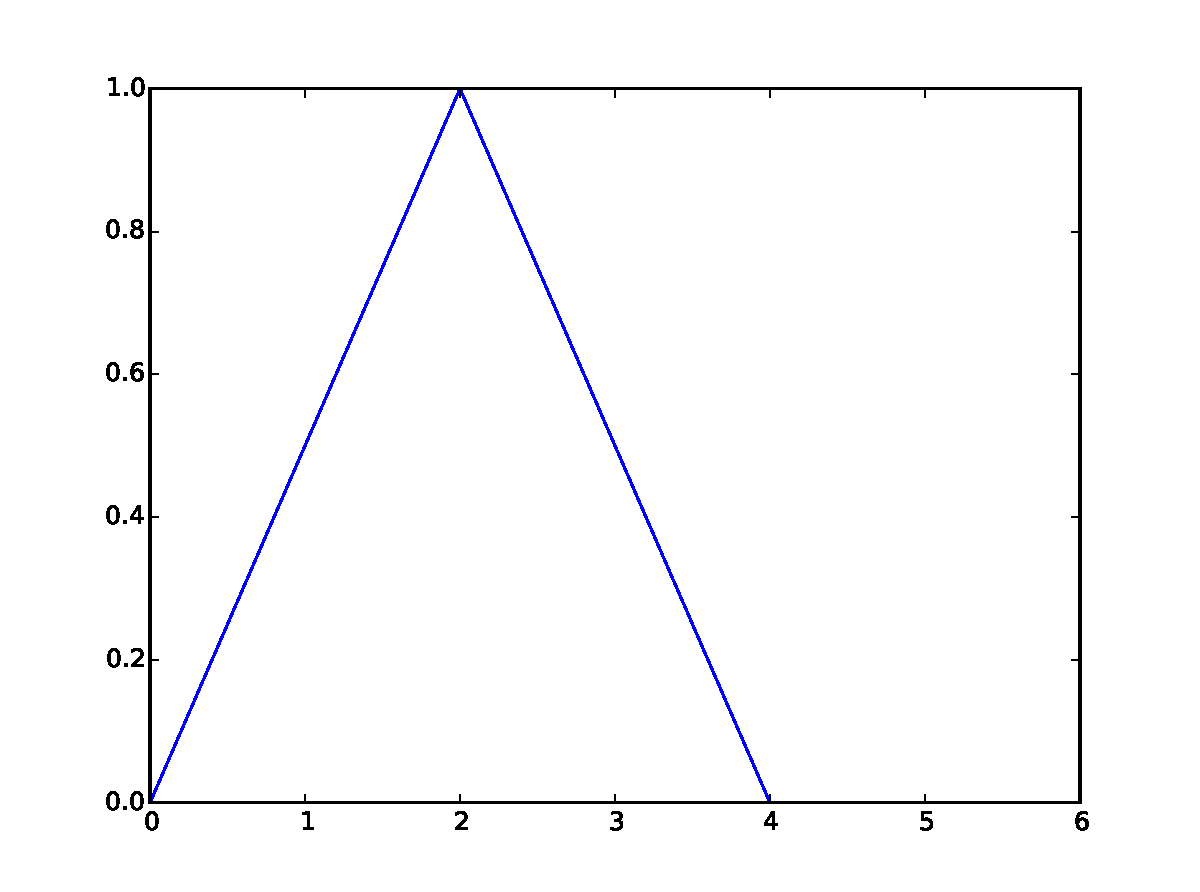
\includegraphics[width=.7\textwidth]{basis_2.pdf}
\end{figure}
\end{columns}
\begin{figure}
\centering
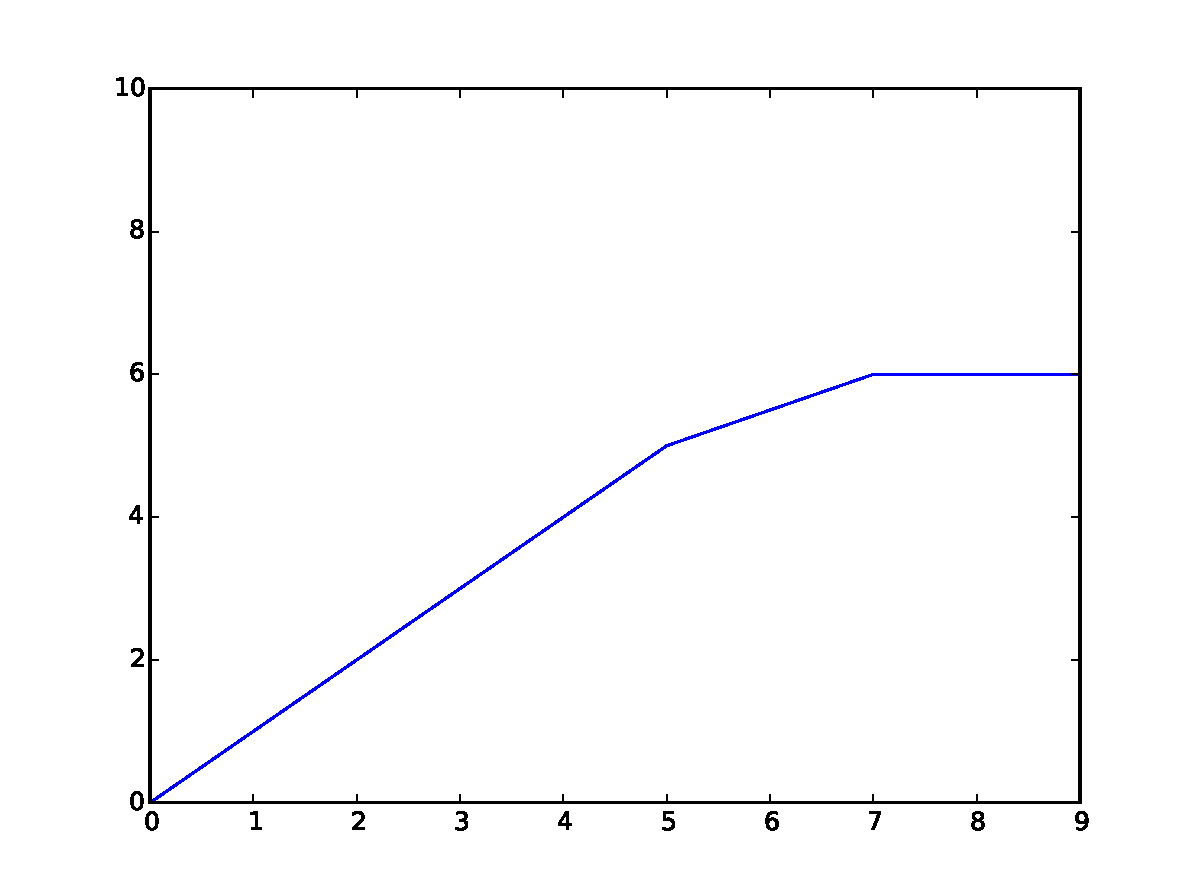
\includegraphics[width=.5\textwidth]{plf_2.pdf}
\end{figure}
\end{frame}

\begin{frame}
\frametitle{Approach}
Forget about historic information temporarily and use linear programming,
\begin{equation}
\begin{array}{ll}
\max\limits_{\mathbf{\mathcal{X}_t}} &\mathbb{E}_{\xi}\left(\sum\limits^T_{t=1} \sum\limits^J_{j=1} v_j X_{t,j} L(\xi)\right)\\
s.t. & 0\leq X_{t,j} L(\xi) \leq \xi_{t,j}\\
& \sum\limits_{t=1}^T\sum\limits^J_{j=1} A X_{t,j} L(\xi) \leq 2\mathbf{c} - \mathbb{E}(\sum\limits_{t=1}^T \sum\limits^J_{j=1} A X_{t,j} L(\xi))\\
&\forall \xi \in \Xi,t=1,\ldots,T
\end{array}
\label{originthird}
\end{equation}
where $L(\xi)$ lift $\xi$ to values of basis functions,and $X_{t,j}$ is actually coefficient matrixes.
\end{frame}

\begin{frame}
\frametitle{Details in above equation}
\begin{itemize}
\item It's not hard to prove that shapes of $X_{t,j} L(\xi)$ will be something like we required. So we can get booking limits from maximum of $X_{t,j} L(\xi)$ and then implement polices.
\item $\mathbf{c} - \mathbb{E}(\sum\limits_{t=1}^T \sum\limits^J_{j=1} A X_{t,j} L(\xi))$ is added to ensure that we can make use of resources as much as possible. In fact, $\sum\limits_{t=1}^T\sum\limits^J_{j=1} A X_{t,j} L(\xi) \approx 2\mathbf{c} - \mathbb{E}(\sum\limits_{t=1}^T \sum\limits^J_{j=1} A X_{t,j} L(\xi))$.So expectations of used resources will be $c$.
\end{itemize}
Now we turn to problems of making use of historic information.
\end{frame}
\begin{frame}
\frametitle{Historic information}
A usual way is using linear combinations of historic information,that is, $X(\xi^{t-1},\xi_t)=X_1(\xi_t)+X_2(\xi^{t-1})$. However,it couldn't give a good results,as we have constraints $X(\xi^{t-1},\xi_t) \leq \xi_t$ and $X_1(\xi_t) \leq \xi_t$. It suggests that we cannot use linear way to approach the multivariate function.

\begin{figure}
\centering
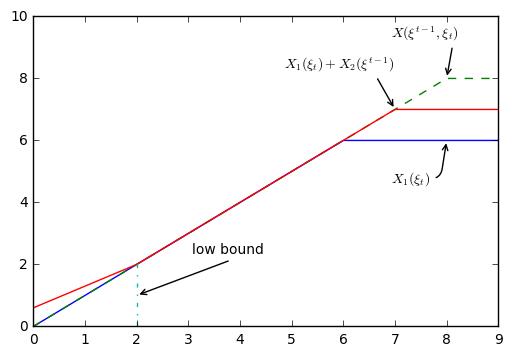
\includegraphics[width=.5\textwidth]{plus.png}
\caption{Cases of low bound of $\xi_t \geq 0$, we can see the limitation of the method}
\end{figure}
\end{frame}
\begin{frame}
\frametitle{Historic information}
\begin{itemize}
\item
Remember that we didn't give $L(\cdot)$ a specific form.
\item
Now we are going to set elements of $L(\cdot)$ be functions of two variables and deal with problems in 2-dimension seems like in 1-dimension.
\item
Simple triangulations are required to approach with piecewise linear functions in 2-dimension.
\end{itemize}
\begin{figure}
\centering
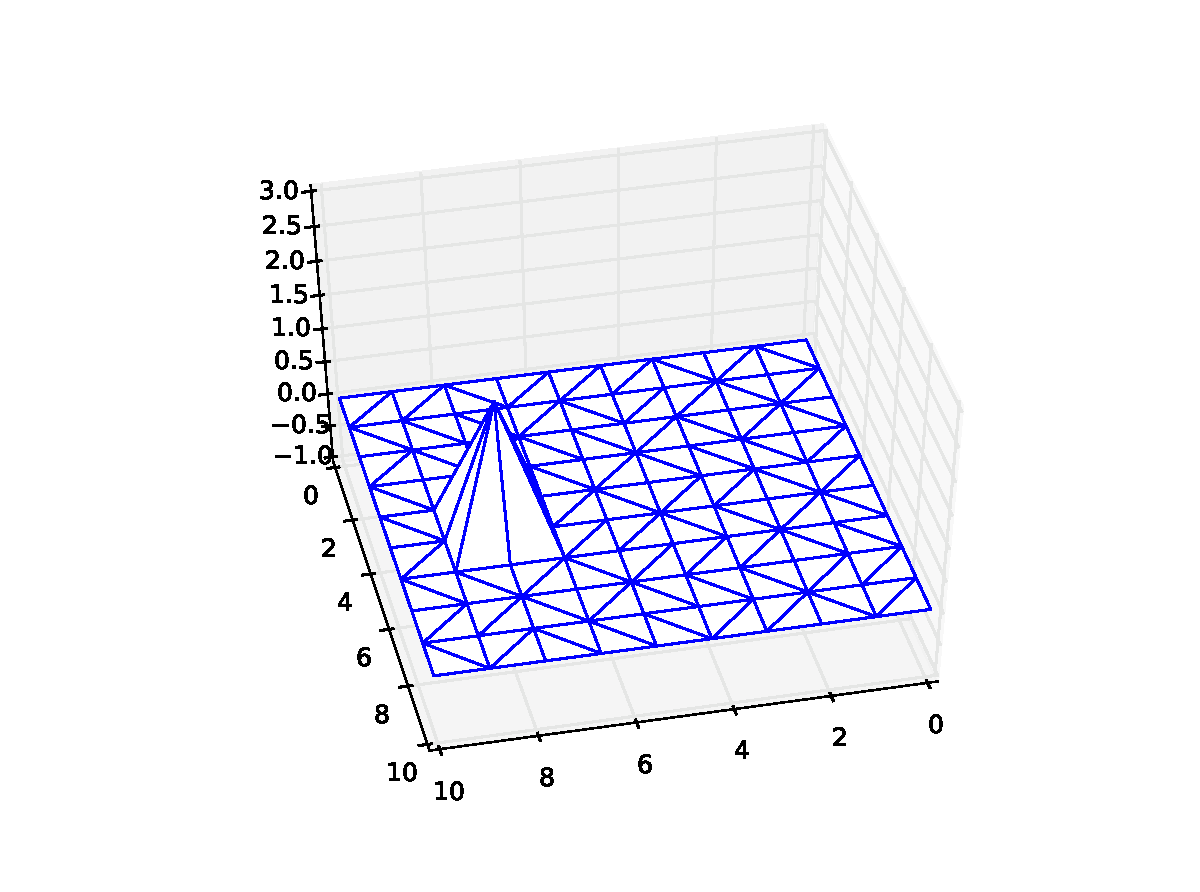
\includegraphics[width=.5\textwidth]{basis_3.pdf}
\caption{a basis function in 2-dimension}
\end{figure}
\end{frame}

\begin{frame}
\frametitle{Solving Nonlinear Optimization in 2-d with Linear Programming}
\begin{itemize}
\item What we are actually doing is solving a nonlinear optimization in 2-dimension with linear programming !
\end{itemize}
\end{frame}

\begin{frame}
\frametitle{Computational Results}
\begin{figure}
\centering
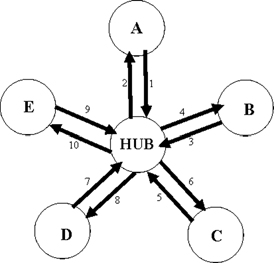
\includegraphics[width=.5\textwidth]{resolve.png}
\caption{Network in Re-solving stochastic programming models for airline
revenue management}
\end{figure}
\end{frame}

\begin{frame}
\frametitle{Computational Results}
Re-solving:

%
%\begin{equation}
%\begin{array}{ll}
%\max & f^T \mathbb{E}\left[\min\left\{x,\sum\limits^{H}_{m=1}\xi^m\right\}\right]
%& Ax\leq c,x\in \mathbb{Z}_+
%\end{array}
%\begin{array}{ll}
%\max & f^T\mathbb{E}\left[\min\left\{x,\sum\limits^{H}_{m=h+1}\xi
%\end{array}
%\end{equation}

\end{frame}

\begin{frame}
\frametitle{Computational Results}
\centering
\begin{table}
\begin{tabular}{ccc}
No re-solving &Uniform re-solving&Trick re-solving\\
\hline
415410 &419262& 421894 
\end{tabular}
\caption{Results from re-solving paper}
\end{table}
\begin{table}
\begin{tabular}{cccc}
Stages& 5 & 10 & 20 \\
\hline
& 420364 & 419474&418527
\end{tabular}
\caption{Results from our paper}
\end{table}
And actually our method are much faster and can also use re-solving to promote results and use ideas from Reductions of Approximate Linear Programs for Network Revenue Management!
\end{frame}

\begin{frame}
\frametitle{Computational Results}
\begin{itemize}
\item
Number of variables is only $O(T\times J)$.
\item Our method is less customize and more intelligent.
\item
Decision rule approach can give a fractional estimation of booking limits.After rounding, we can use Zhang's method to give a better solution in need of a higher accuracy.
\end{itemize}
\end{frame}
\begin{frame}
\frametitle{Future Work}
\begin{itemize}
\item As we can see, we can generalize original problems into higher dimension. In the meantime, we have to face curse of dimensionality.
\item Not only $X(\sum\limits_{\tau=1}^{t-1} \xi_\tau,\xi_t)$ but also $X(\max\limits_{\tau=1,\ldots,t-1}\xi_\tau,\xi_t)$ is available. It hints us that the
methodology is suitable to approximate dynamic programs in other scenrios.
\item Rounding policy.
\end{itemize}
\end{frame}
\end{document}
